\section{Systemdesign}
\subsection{Navigasjon}
Appen består av to hovedelementer for navigasjon, et bottom-navigation element, og et navigation-drawer element. I tillegg til disse har den en swipe-funksjon når man befinner seg i forsiden, kartsiden og vennesiden. Det vil være mulig å navigere mellom disse tre sidene med bottom-navigation elementet, men også å swipe fra venstre til høyre og motsatt. Tilgjengelig fra de fleste sider vil være en navigation-drawer som brukes til å navigere til resten av appen.

Grunnen til denne oppdelingen er for å skille mellom sider som blir brukt mye og sider som blir brukt lite. Vi har valgt å bruke bottom-navigation og swipe-funksjonen til forsiden, kartsiden og vennesiden, fordi de er sentrale og brukes nesten hver gang appen er i bruk. Forsiden er det samme som oversiktssiden, så dette vil være landingssiden når brukeren logger inn. I navigation-drawer elementet kan man blant annet navigere seg til innstillinger og enhetskatalogen.

\subsubsection{Flyt}

\begin{figure}[H]
    \centering
    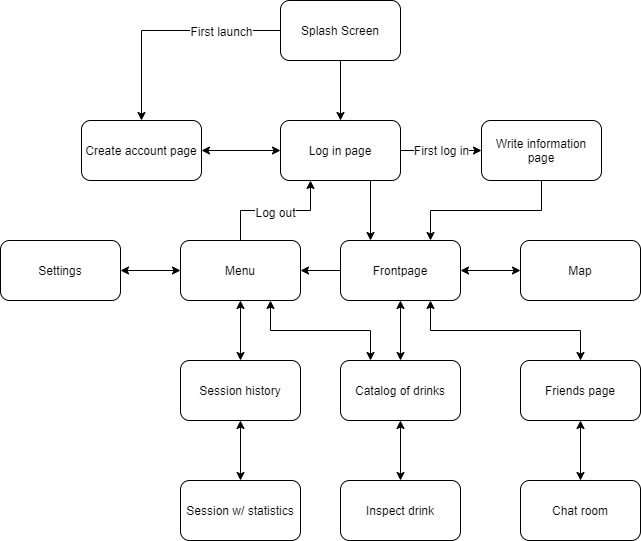
\includegraphics[scale=0.5]{images/lille_promille_float_diagram.drawio.png}
    \caption{Skisse som viser hvor man kan navigere seg til fra hvilke sider i appen.}
\end{figure}

\subsubsection{Navigation Pattern}
Bla bla bla

\subsection{Teknisk oppbygging}
Blablabla

\subsubsection{Lagring og uthenting av data}
For å lagre brukerdata benyttes Firestore. Dette gjøres via Firebase, her lagres brukere i en "user" collection. Hver bruker lagres med en UUID som autogeneres fra Firebase. 

Brukerinformasjonen lagres rett i dokumentet til brukeren, mens enhetskatalogen og økt historikken lagres i collections på brukeren. 
Disse 

Når en bruker logger inn hentes dataen til brukeren ved å bruke Firebase UUID'en, da oppdateres først dokumentreferansen så brukes denne til å hente riktig data, brukerdaten blir da lagret in UserDatabaseHandler, denne dataen hentes da senere i settingsFragment. 

Når brukeren logger inn gjøres det en sjekk på om det er en ny bruker, hvis det er en ny bruker hentes ikke dataen. 
Da legges det til en bruker med tomme verdier til database. 

Når brukeren navigerer ut av settingsFragment hentes den oppdaterte dataen fra Firebase.

\subsubsection{Brukerhåndtering}
Håndtering av brukere gjøres gjennom Firebase.

Brukeren får via appen muligheten til å lage en ny bruker, oppdatere og slette brukeren.

En bruker består av feltene:
\begin{itemize}
    \item age
    \item height
    \item weight
    \item gender
    \item username
    \item currentSession
    \item weight
\end{itemize}

En sessionHistory collection og en alcoholUnitCollection.

\subsection{Ressurser}
\subsubsection{Services}


\subsubsection{Fragmenter}

\subsubsection{Bilder}
Bilder i appen vil bestå av ikoner, logoer, emojier og eventuelt profilbilder. Ikonene brukes til å veilede brukeren der det er raskere å oppfatte ikonet enn å det er å lese teksten, for eksempel til navigasjonspunktene i bottom-navigation og navigation-drawer. Ikonene er en blanding av lånte og egenskapte ikoner som følger design prinsippene til Material Design dokumentasjonen(1). Logoen lager vi selv, og vi skal ha variasjoner av logoen 

\subsubsection{Biblioteker}